\section{Experimentacion}
\subsection{Busqueda exhautiva}
Para comenzar la experimentación y tener una idea aproximada sobre los mejores valores de los parámetros del modelo utilizamos la técnica de \textit{grid search} o búsqueda exhaustiva. Siempre corrimos con un \textit{holdout set} de validación del 50\% del dataset completo, para poder simular la performance de nuestra implementación con datos nuevos que no se usaron en el entrenamiento. 

En el ejercicio uno, la búsqueda trata de minimar la suma de errores totales del set de validación, mientras que en el ejercicio dos se hace lo mismo pero al ser un problema de regresión, se define como error cuando el output de la red y el target es mayor a un \textit{epsilon} definido. 

La implementación es bastante simple, lo que hacemos es pasar por parametro una lista con todos los posibles para parametros y el algoritmo corre un ciclo, donde en cada ciclo prueba con un parametro distinto guardandoce el mejor modelo para finalmente imprimirlo por la consola. 

Además tuvimos en cuenta el componente de inicialización aleatorio de la red neuronal. Para esto decidimos correr 3 veces cada set de parámetros y quedarse con el mejor. 

Los parámetros que variamos fueron los siguientes:
\begin{itemize}
\item \textbf{Learning Rate}
\item \textbf{Momentum}
\item \textbf{Incremental o Batch}
\item \textbf{Configuración/Cantidad de capas y neuronas}
\end{itemize}

Una vez obtenidos los mejores parámetros, continuamos los experimentos variandolos a mano y analizando los resultados. Esto se explicará en la sección siguiente.

El algoritmo es el siguiente:

\begin{lstlisting}[caption=grid\_search]
def grid_search(param_grid):
	grid = ParameterGrid(param_grid)
	best_error = None
	best_params = None
	print "Ejercicio "+str(param_grid["1"])
	print len(grid), "modelos distintos"
	i = 0
	print "i 	error(training, validacion)"
	start = timer()
	for params in grid:
	    e = train(params['1'], params['2'], params['3'],params['4'],params['5'],params['6'],params['7'],
	    	params['8'],params['9'],params['10'],params['11'], True )
	    print i, "	", e
	    i += 1
	    if i%50 == 0:
	    	end = timer()
	    	print int((end-start)/60), " min"
	    if best_error == None or e < best_error:
	    	best_error = e
	    	best_params = [params['1'], params['2'], params['3'],params['4'],params['5'],params['6'],params['7'],params['8'],
	    	params['9'],params['10'],params['11']]
	print "MEJOR ERROR Y MODELO EJERCICIO "+str(param_grid["1"])
	print "training, validacion:", best_error
	print "parametros:", best_params
	end = timer()
	print int((end-start)/60), " min"
\end{lstlisting}

Y la forma de instanciarlo es la siguiente:

\begin{lstlisting}[caption=Instanciacion]
param_grid = {'1': [1],"2":['./datasets/tp1_ej1_training.csv'],"3": [None], "4":[0.1], "5": [200], 
			"6":[0.001,0.01,0.1,0.5, 0.005, 0.2, 0.3, 0.4], "7":[0.1,0.3,0.5, 0.7, 0.9], "8": [0.70], 
			"9": [0,1], "10":[0], "11":[[5],[10],[15],[20],[25],[15,15],[5,5],[10,10]]}
\end{lstlisting}


\subsection{Ejercicio 1}

Observamos que agregar capas no garantiza la convergencia y, cuando lo hace, provoca que las salidas oscilen abruptamente y tarde mas epocas, por lo que optamos por utilizar \textbf{dos capas ocultas} como compromiso entre tiempo y calidad de solucion. 


En cuanto al numero de unidades por capa, ejecutamos el grid\_search 10 veces y en total encontramos que una buena solucion es:

\begin{enumerate}
\item epsilon: 0.1
\item tau: 200
\item etha: 0.01
\item momentum: 0.9
\item holdoutRate: 0.7
\item modo: Incremental
\item unidades por capa: 5 y 5
\end{enumerate}

Y para esta obtuvimos los siguientes graficos.


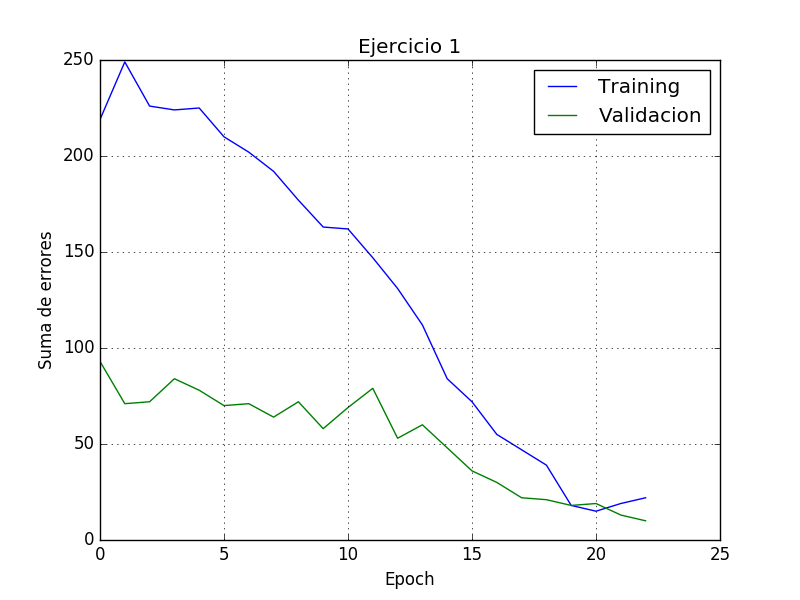
\includegraphics[scale=0.4]{img/ej100109155sum}
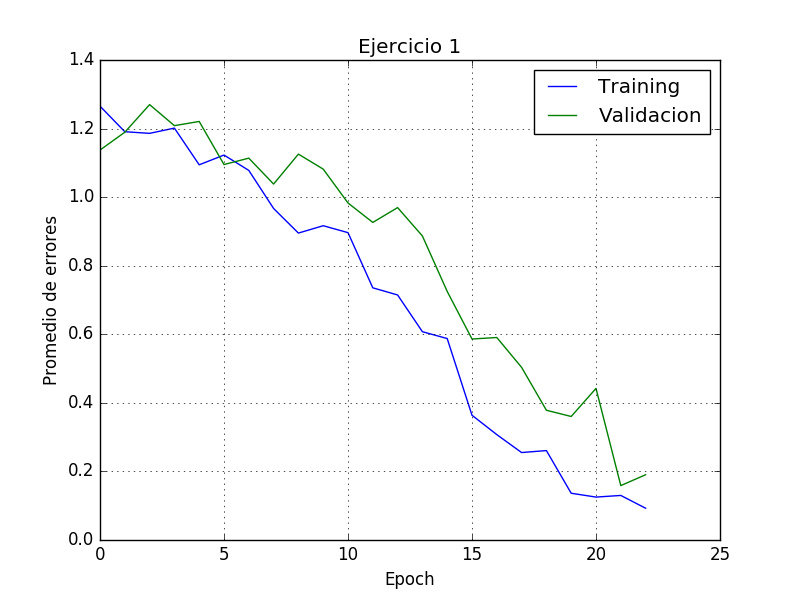
\includegraphics[scale=0.4]{img/ej100109155mean}

En estos graficos podemos ver que en el promedio, al promediar la cantidad de casos se puede ver que el trainning da mejor que validacion. Al mismo tiempo en la suma de errores la validacion da menor porque hay menos casos de entrada. 
Por otro lado, vemos que si mantenemos la cantidad de epocas podemos caer en overfitting porque el error de trainning podria seguir disminuyendo pero el de validacion no.
Un detalle importante es que esta arquitectura, cuando convergue, lo hace rapido. Como se pueder ver en este ejemplo de muestra que converge en un poco mas de 20 epocas.

De todas formas analizando los graficos tras varias corridas vimos que no siempre convergia esta solucion.
Como el campo de busqueda es pequeno, probamos multiples veces diferentes configuraciones de neuronas con numeros de 2 a 15 neuronas por capa para tener una evidencia estadistica de que sucede al variar este parametro. Con ello corroboramos que la solucion arrojada por el algoritmo de busqueda estaba cerca de un resultado optimo al ver las variaciones de diferentes medidas de error. 

Las medidas de error que tomamos fue el numero de unidades con error, el error total, el promedio de error, condicion de terminacion de aprendizaje, es decir, si termino por error menor a epsilon o por limite de epocas. En particular, por la naturaleza del problema, nos interesa ver la Precisión y el Recall, o dicho de otra manera, el indice de falso positivo y falso negativos. 

Como medida utilizaremos la Media armónica donde 

$Media armonica=2*precision*recall/(precision+recall)$

$precision=true positive/(true positive+false positive)$

$recall= true positive/(true positive+false negative)$


Para determinar el valor de la primer capa, elegimos aquellas configuraciones que nunca terminen debido al limite de epocas. Luego, en base a la cantidad de unidades con error y el error total cometido, las clasificamos en este orden. 
En particular, obtuvimos que las configuraciones de [8,7] y [9,5] arrojan buenos resultados (en base a la suma de errores y el promedio).

Podemos ver a continuacion algunos graficos obtenimos variando los parametros con 8 y 7 capas.

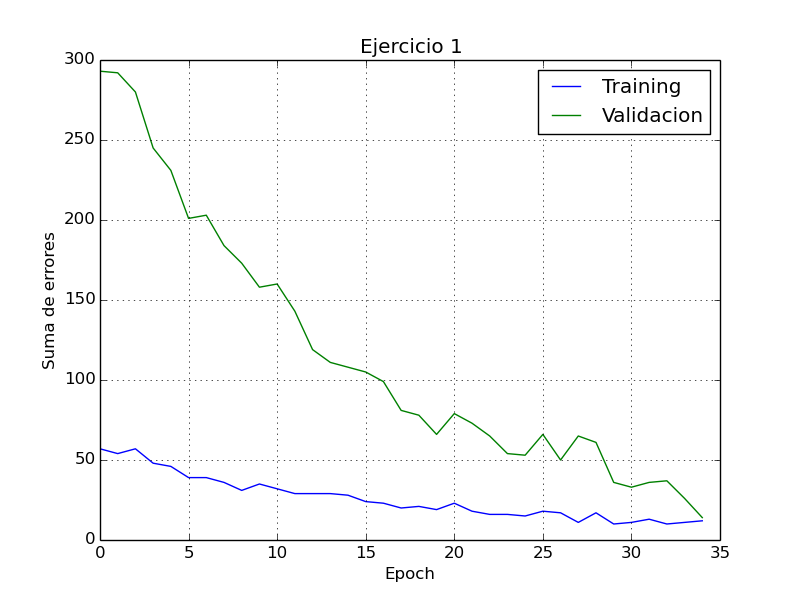
\includegraphics[scale=0.4]{img/ej100207187sum}
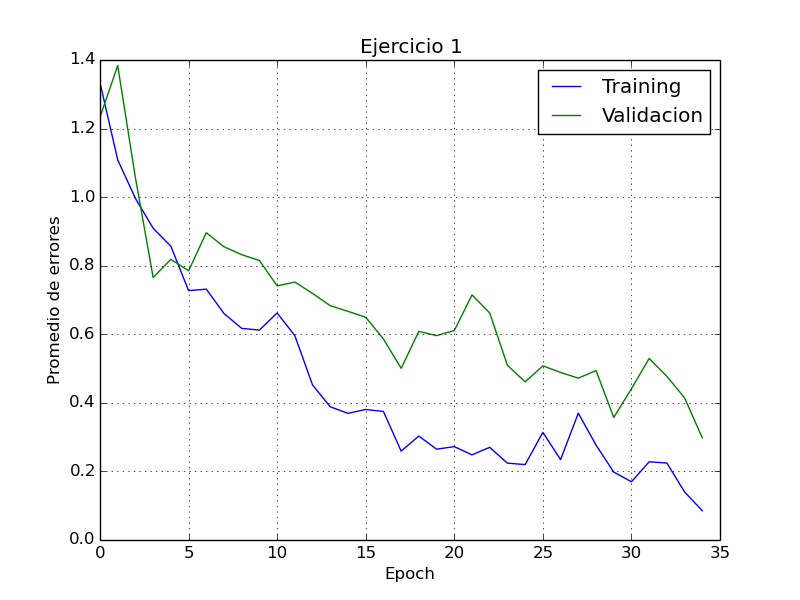
\includegraphics[scale=0.4]{img/ej100207187mean}

En particular este grafico fue el mejor de los graficos que obtuvimos variando los parametros para esta cantdiad de capas. Y los parametros son:
\begin{enumerate}
\item epsilon: 0.1
\item tau: 200
\item etha: 0.02
\item momentum: 0.7
\item holdoutRate: 0.7
\item modo: Incremental
\item unidades por capa: 8 y 7
\end{enumerate}

Se puede ver en estos graficos que a simple vista, el promedio de errores tiene un mayor numero de oscilaciones. Tambien vemos que compardo a los graficos del [5,5], este converge en una cantidad de epocas mayor.

Podemos ver a continuacion algunos graficos obtenimos variando los parametros con 9 y 5 capas.


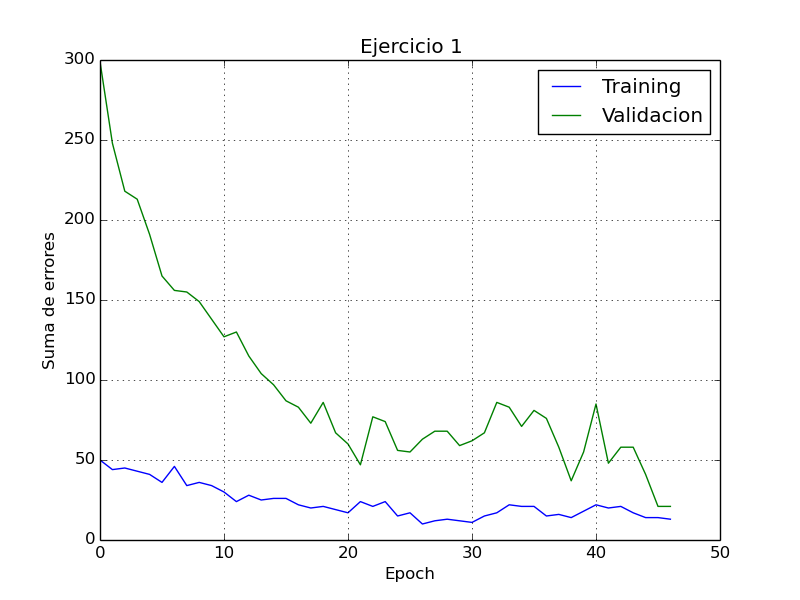
\includegraphics[scale=0.4]{img/ej100505195sum}
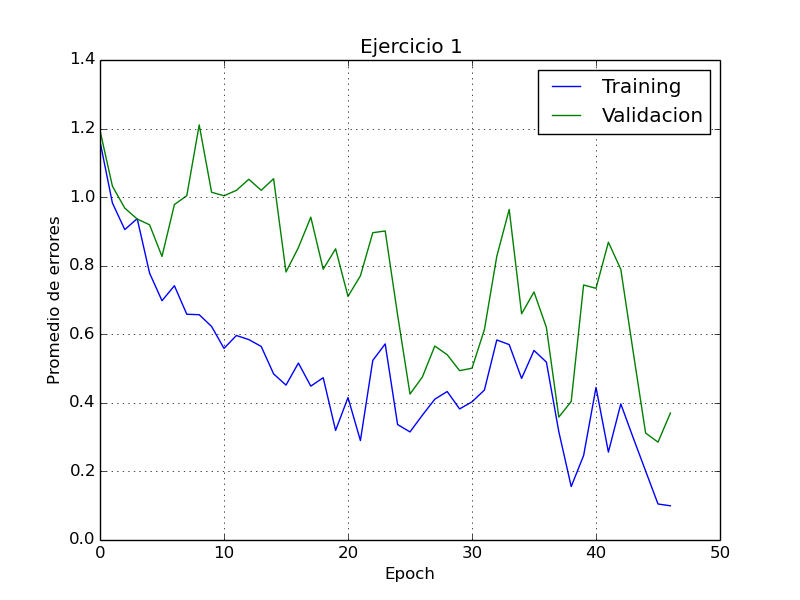
\includegraphics[scale=0.4]{img/ej100505195mean}


En particular este grafico fue el mejor de los graficos que obtuvimos variando los parametros para esta cantdiad de capas. Y los parametros son:
\begin{enumerate}
\item epsilon: 0.1
\item tau: 200
\item etha: 0.05
\item momentum: 0.5
\item holdoutRate: 0.7
\item modo: Incremental
\item unidades por capa: 9 y 5
\end{enumerate}

Se puede ver en estos graficos que el promedio de errores es bastante variado y que al igual que con [8,7] la cantidad de epocas es mayor que [5,5].

Notamos que el numero de neuronas en la ultima capa permite que la salida se ajuste al resultado mientras que la primer capa realiza el grueso del esfuerzo de generalizacion. Al contrario de lo que esperabamos, incrementar el numero de unidades de la ultima capa no mejora el resultado, si no que lo empeora debido a que le lleva un mayor numero de epocas para converger (cuando lo hace). Pocas neuronas en la capa final mostraron experimentalmente que proveen una buena solucion.

Por lo mencionado anteriormente, analizamos el valor del Mean Armonic para una muestra que reservamos del dataset original (que no se uso en el entrenamiento) y obtuvimos que el caso de [8,7] capas da un valor del 0.94527, el caso de [9,5] capas da un valor del 0.9508 y el caso de [5,5] capas da un valor de 0.97.


En conclusion, decidimos elegir como modelo el de 5 y 5 capas dado el Mean Armonic da mas cercano a 1, es un modelo con pocas capas entonces tiene una velocidad de procesamiento mayor.
Ademas, analizamos los histogramas para ver la cantidad de equivocaciones a la hora de predecir si un cancer es benigno o maligno obteniendo para el caso de [5,5]:

\begin{center}
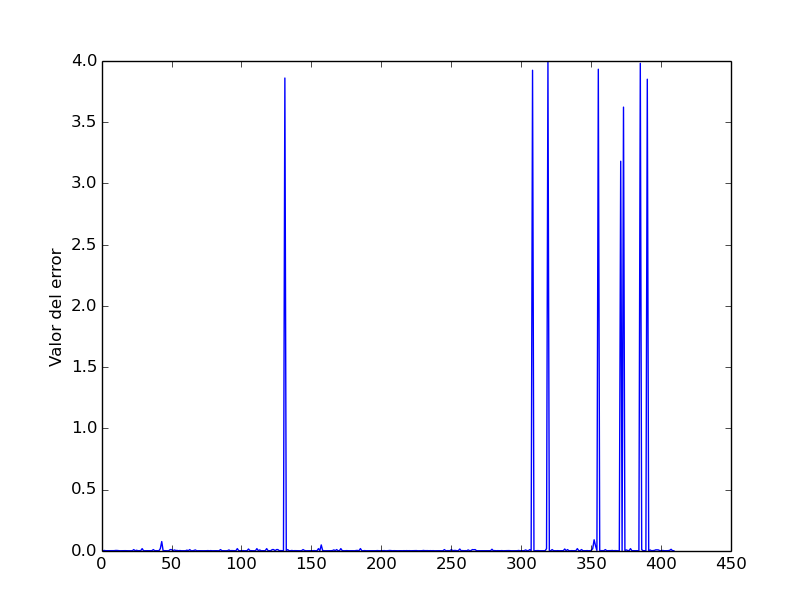
\includegraphics[scale=0.5]{img/histogramaej155}
\end{center}

y para el caso de [9,5] el siguiente grafico

\begin{center}
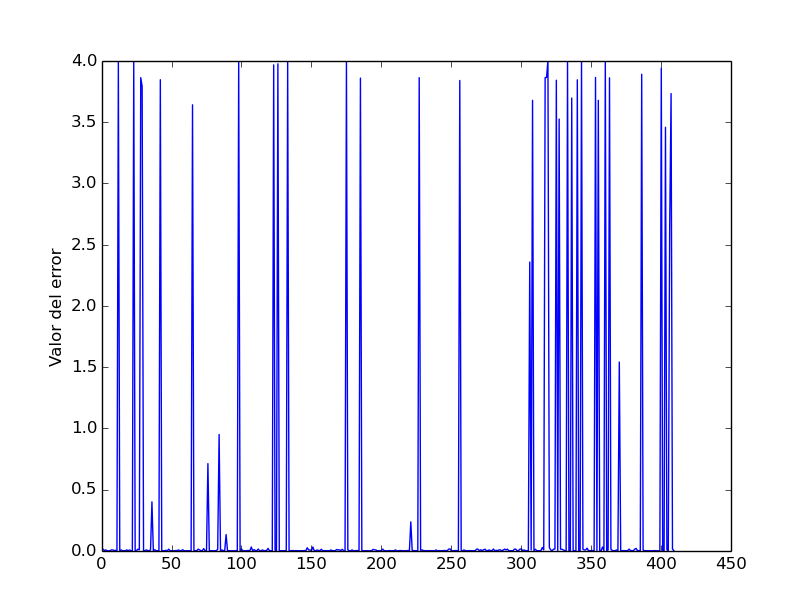
\includegraphics[scale=0.5]{img/ej195_histograma}
\end{center}

Concluyendo, podemos ver que en el grafico de [5,5] capas la cantidad de equivocaciones es 8, siendo este un numero menor que el de [9,5] capas. Tener en cuenta que la cantidad de muestras es de 400.

\subsection{Ejercicio 2}

Al igual que en el ejercicio 1, en este ejercicio se corrio el algoritmo de grid\_search 10 veces y en total encontramos dos  soluciones buenas. 

La primera:

\begin{enumerate}
\item epsilon: 0.01
\item tau: 200
\item etha: 0.005
\item momentum: 0.9
\item holdoutRate: 0.7
\item modo: Incremental
\item unidades por capa: 5
\end{enumerate}

Y para esta obtuvimos los siguientes graficos.

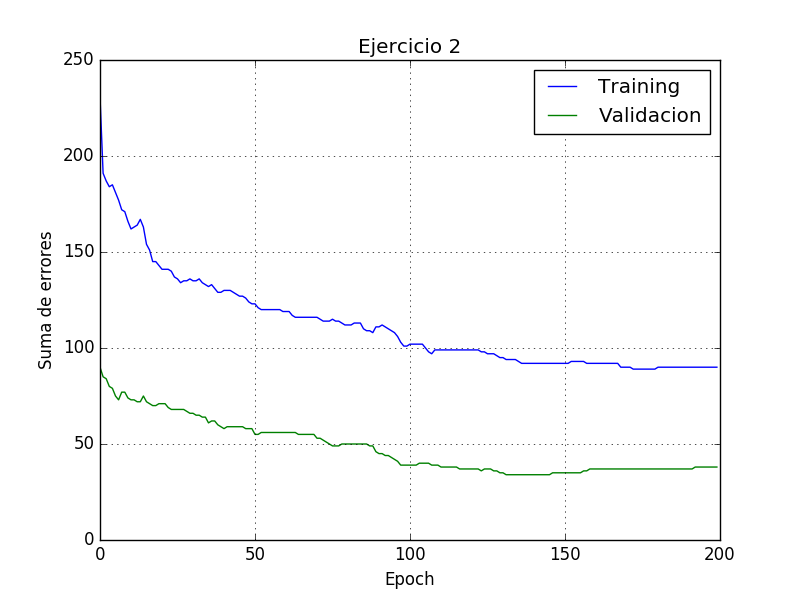
\includegraphics[scale=0.4]{img/ej200050915sum}
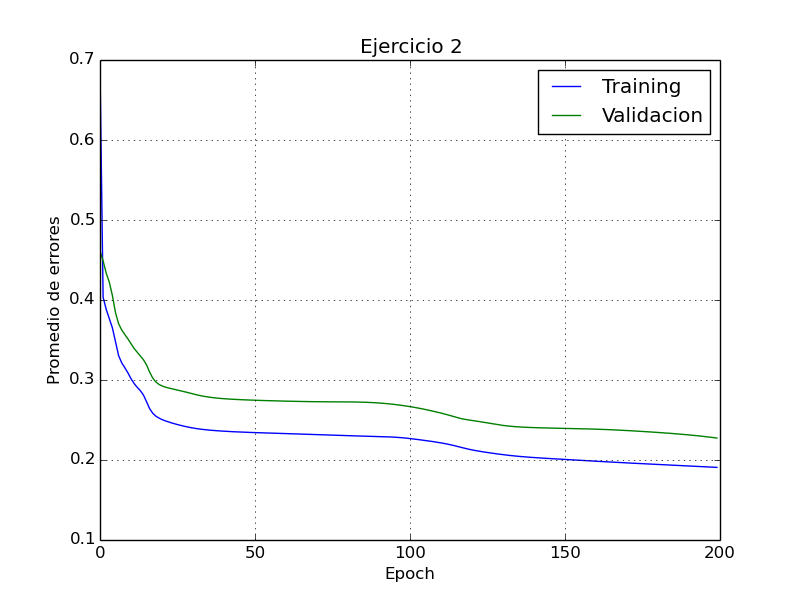
\includegraphics[scale=0.4]{img/ej200050915mean}

Se puede ver en estos graficos que en el grafico de suma de errores las dos curvas se comportan igual, esto es porque es un problema de regresion y las funciones utilizadas son linealmente dependiente, es decir, la salida es proporcional a la entrada.

Un detalle importante es que en este grafico vemos como la curva \textbf{no se plancha}, y este era un problema que teniamos en la mayoria de los casos de 2 capas. 

La otra red que nos arrojo el grid\_search es la siguiente:

\begin{enumerate}
\item epsilon: 0.01
\item tau: 1000
\item etha: 0.01
\item momentum: 0.6
\item holdoutRate: 0.85
\item modo: Incremental
\item unidades por capa: 8 y 5
\end{enumerate}

Con esta arquitecutura generamos las siguientes imagenes:

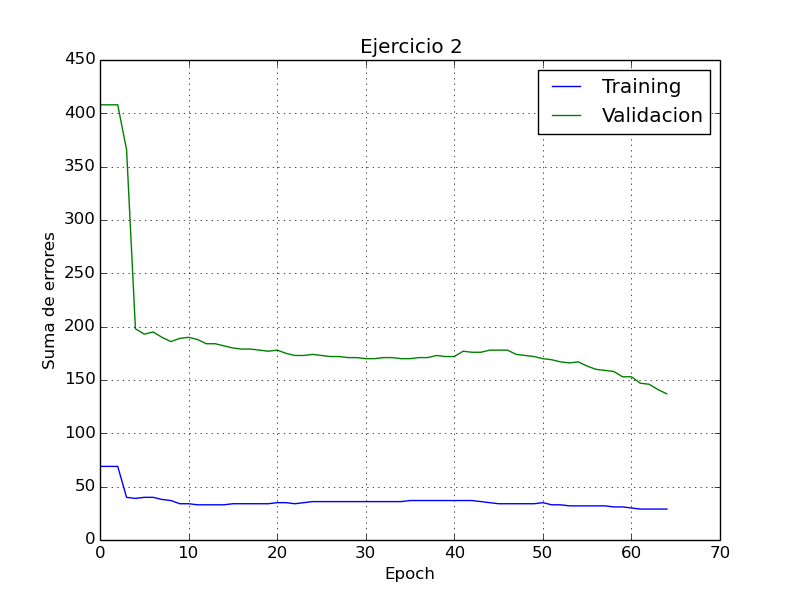
\includegraphics[scale=0.4]{img/asum}
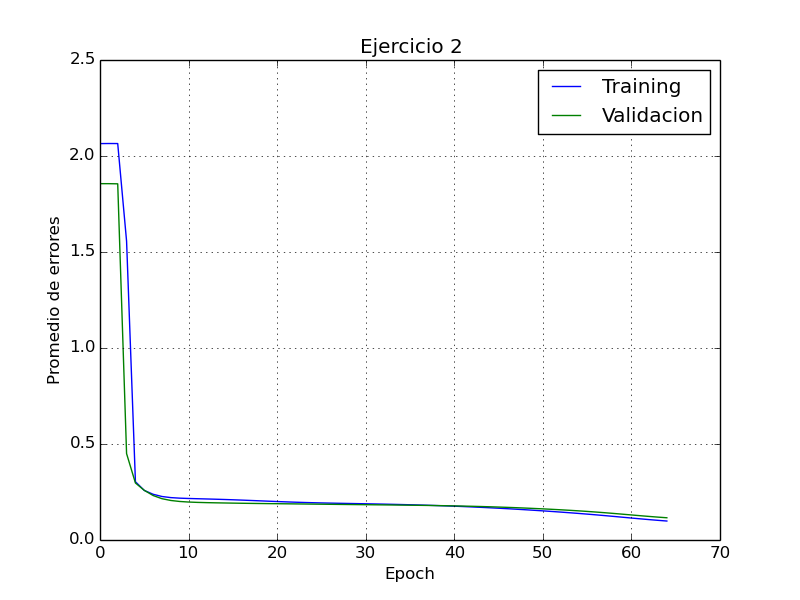
\includegraphics[scale=0.4]{img/bmean}

Se puede ver en estos graficos que la suma de errores se mantiene constante en un intervalo, es decir, parece que tiene una asintota, en otras palabras, \textbf{se plancha}. Esto es un error tipico encontrado en las ejecuciones de 2 capas. Creemos que esto es debido a la funcion de activacion dado que, utilizamos una sidmoide y entonces esta tiene este comportamiento.

Por otra parte, al igual que en el ejercicio anterior, probamos a mano cambiar los valores de los parametros pero de todas formas no encotnramos nada mejor. En general todos los resultados que obtuvimos fueron similar a este:

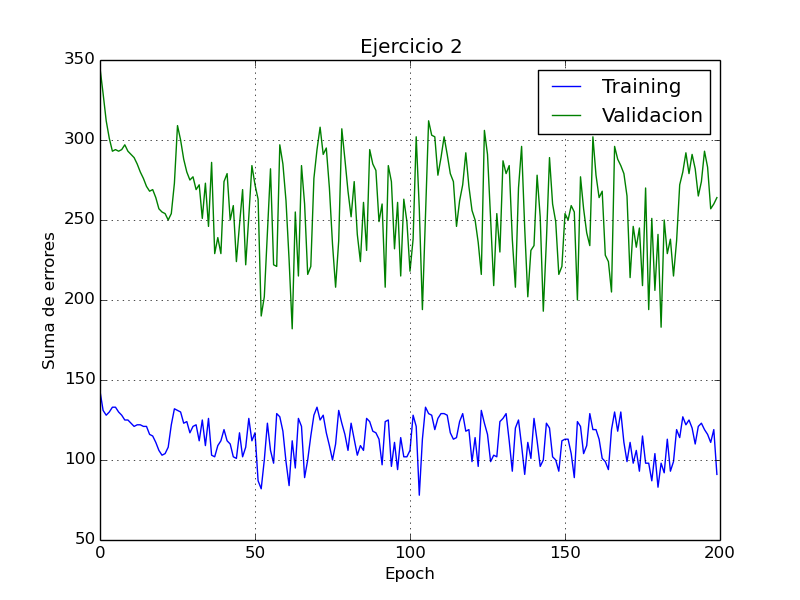
\includegraphics[scale=0.4]{img/ccsum}
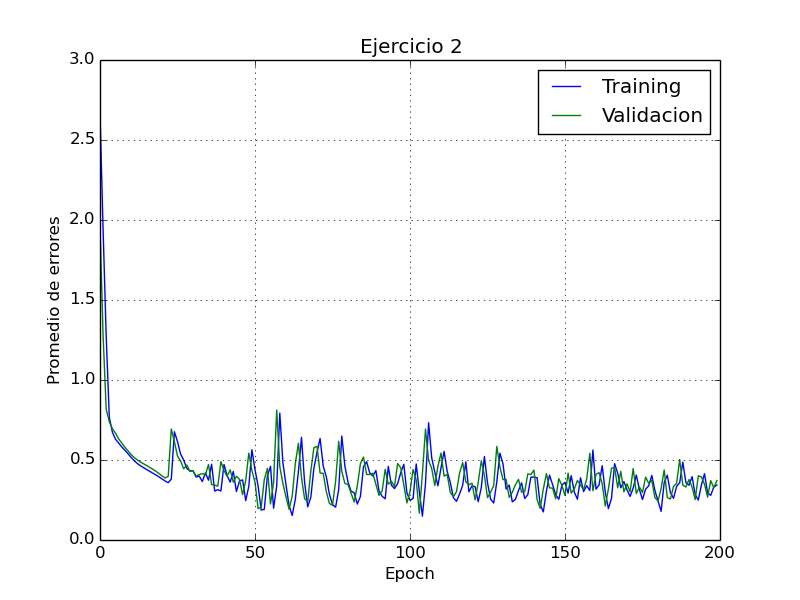
\includegraphics[scale=0.4]{img/bbmean}

estos graficos corresponden a los siguientes parametros:

\begin{enumerate}
\item epsilon: 0.01
\item tau: 200
\item etha: 0.1
\item momentum: 0.9
\item holdoutRate: 0.7
\item modo: Batch
\item unidades por capa: 15
\end{enumerate}
En estos graficos se puede ver una notable inestabilidad por parte de la red (se ve en ambos graficos). Tambien podemos ver que, la suma de errores se mueve en un intervalo fijo, es decir, no esta desendiendo. 

Como se podra ver en los graficos elegimos el primer modelo porque es el que mas desciende y tambien tiene menor cantidad de capas, por lo tanto procesamiento mas rapido. Tambien vemos que la derivada de la funcion de promedio de errores nunca es cero, esto quiere decir que el modelo aprende.


Para este modelo elegido, hicimos unos graficos de dispercion. 
En este grafico se puede ver en el eje \textbf{y} el valor predicho y en el eje \textbf{x} el valor objetivo. En general lo ideal es concluir en un grafico como el siguiente:

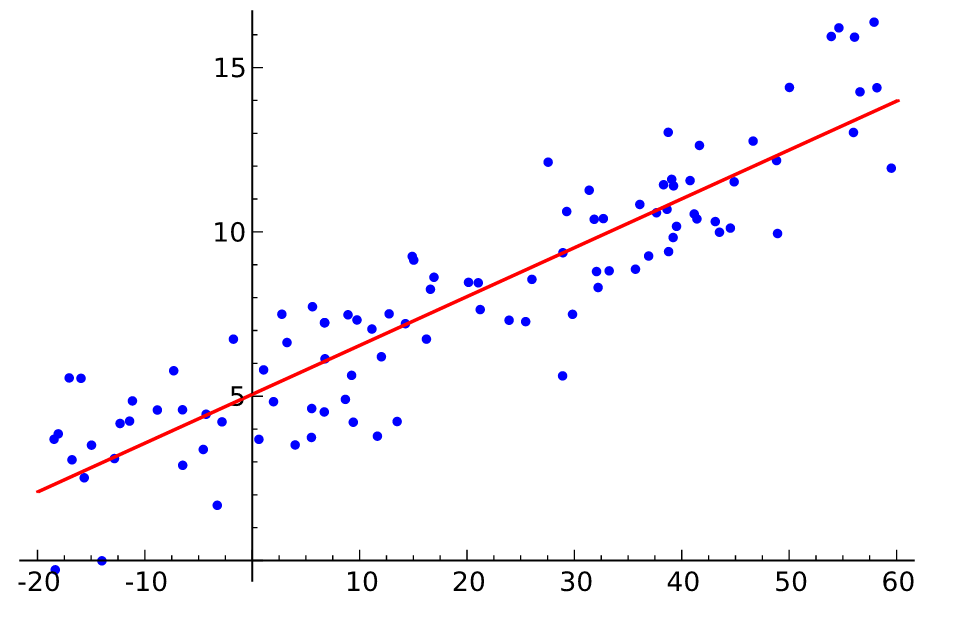
\includegraphics[scale=0.4]{img/regresionperfecta}

Con nuestra arquitectura obtuvimos los siguientes graficos:

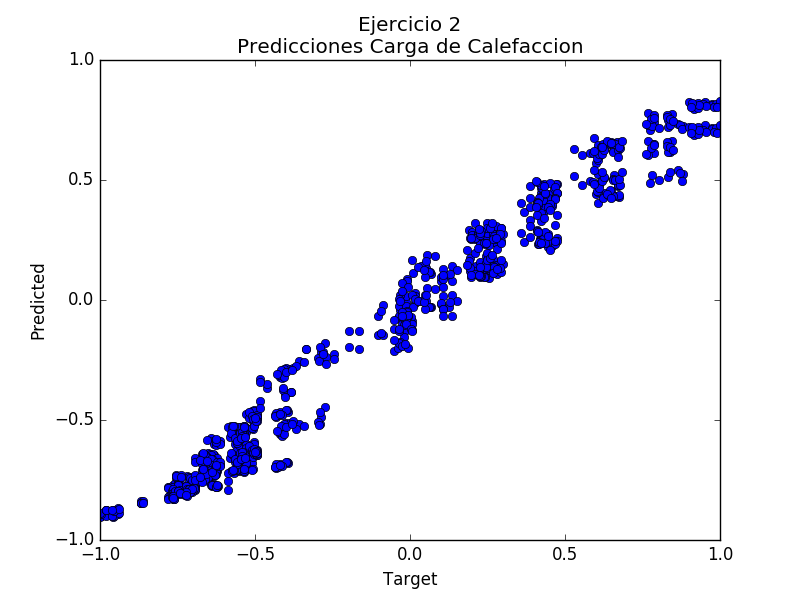
\includegraphics[scale=0.4]{img/ej2-calef}
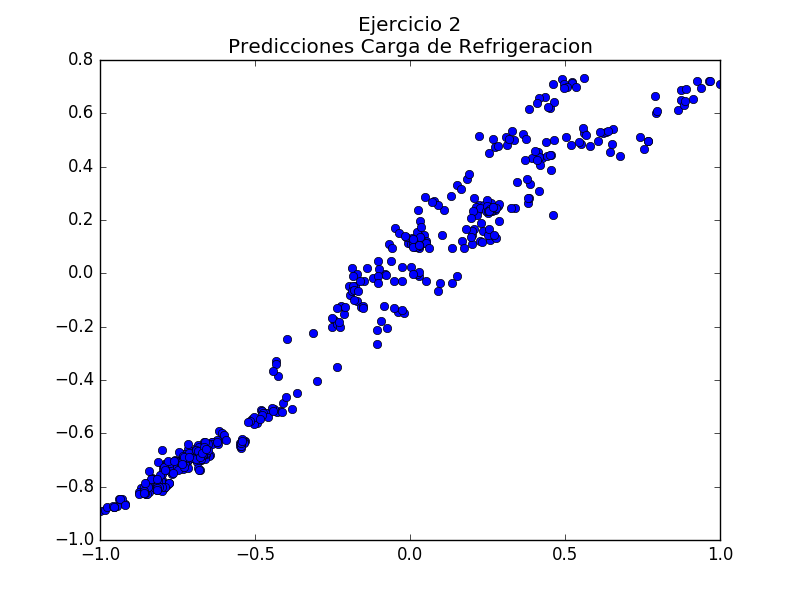
\includegraphics[scale=0.4]{img/ej2-refrig}


En estos graficos notamos que son similares a lo ideal, sin caer en un overfitting, los puntos obtenidos se acercan a la recta Y=X, lo que quiere decir que los valores aprendidos se acercan mucho al objetivo.
Como se explico en las secciones anteriores el output fue normalizado, por esto la escala del grafico va desde -1 a 1 que es el rango de la funcion sigmoide bipolar.

\subsection{Conclusion}

\emph{\color{red} FALTA }
